\chapter{Campos débiles, ondas gravitacionales y principio de acción}

Las ecuaciones exactas de la relatividad general son no lineales, y su forma en componentes puede volverse formidable antes incluso de resolver un solo problema físico. Para la última clase del curso, conviene separar los principios de los detalles de cálculo. Nos preguntaremos cómo quedan las ecuaciones de Einstein cuando el campo gravitacional es débil, identificaremos las ondas contenidas en esa aproximación y, para terminar, veremos cómo las ecuaciones completas del campo caben en un principio de acción sorprendentemente compacto.

Tres preguntas organizan la discusión. ¿Qué significa que un campo gravitacional sea débil? ¿Por qué la teoría débil es lineal, aunque la teoría exacta no lo sea? ¿Y qué efectos físicos distinguen una onda gravitacional de una mera oscilación de las coordenadas?

\section{Una pequeña perturbación de una geometría de equilibrio}

La debilidad es un esquema de aproximación. Si una perturbación adimensional es del orden de \(\epsilon\ll1\), su cuadrado es del orden de \(\epsilon^2\), y un cálculo de primer orden descarta sistemáticamente este último término. El ejemplo conocido es un sistema mecánico que realiza pequeñas oscilaciones en torno al equilibrio. Sus ecuaciones exactas pueden ser no lineales, pero las oscilaciones suficientemente pequeñas obedecen ecuaciones lineales.

En gravedad, el fondo de equilibrio será el espacio-tiempo plano vacío. Partamos de la ecuación de vacío de Einstein:
\begin{equation}
 R_{\mu\nu}-\frac12 g_{\mu\nu}R=0.
 \label{eq:l10-vacuum-einstein}
\end{equation}
Al tomar la traza en cuatro dimensiones se obtiene
\begin{equation}
 g^{\mu\nu}
 \left(R_{\mu\nu}-\frac12 g_{\mu\nu}R\right)
 =R-2R=-R=0,
\end{equation}
por lo que la ecuación de vacío es equivalente a
\begin{equation}
 R_{\mu\nu}=0.
 \label{eq:l10-ricci-flat}
\end{equation}

\begin{figure}[htbp]
\centering
\includegraphics[width=0.68\textwidth]{lecture_10_figure_02.png}
\caption{La ecuación de vacío \(R_{\mu\nu}=0\), destacada al comienzo del argumento de campo débil.}
\lectureframe{00:03:11}
\end{figure}

Aquí, equilibrio significa una solución sin fuentes y sin dependencia temporal. El espacio-tiempo plano es la solución más sencilla de este tipo. Hay que hacer una salvedad esencial: que sea plano no significa que las componentes de la métrica sean iguales a una matriz particular en todos los sistemas de coordenadas. Significa que se pueden elegir coordenadas inerciales en las que
\begin{equation}
 g_{\mu\nu}=\eta_{\mu\nu}.
\end{equation}
Esta distinción entre la geometría y las coordenadas empleadas para describirla pronto se convertirá en la sutileza central.

Imaginemos ahora una fuente violenta, como un sistema binario compacto. Su campo cercano puede ser intenso, pero, lejos de la fuente, la perturbación se propaga y se vuelve pequeña. Entonces, en un sistema de coordenadas adecuado, la métrica puede escribirse como
\begin{equation}
 g_{\mu\nu}(x)=\eta_{\mu\nu}+h_{\mu\nu}(x),
 \qquad |h_{\mu\nu}|\ll1.
 \label{eq:weak-split}
\end{equation}
Se permite que la perturbación \(h_{\mu\nu}\) dependa de las cuatro coordenadas del espacio-tiempo. La condición de campo débil significa que se despreciarán las potencias de orden superior al primero.

\section{Qué sobrevive al primer orden}

El tensor de Ricci completo es demasiado largo para resultar útil en esta etapa. Basta con conocer su estructura. Los símbolos de Christoffel contienen la métrica inversa y una derivada de la métrica, mientras que la curvatura contiene una derivada de un símbolo de Christoffel y un producto de dos símbolos de Christoffel:
\begin{equation}
 \Gamma\sim\frac12 g^{-1}\partial g,
 \qquad
 R\sim\partial\Gamma+\Gamma\Gamma.
 \label{eq:curvature-skeleton}
\end{equation}

\begin{figure}[htbp]
\centering
\includegraphics[width=0.84\textwidth]{lecture_10_figure_03.png}
\caption{La descomposición de campo débil y la construcción esquemática
\(R\sim\partial\Gamma+\Gamma\Gamma\). La notación muestra los órdenes en
\(h\) sin desarrollar todos los índices.}
\lectureframe{00:10:17}
\end{figure}

La métrica inversa se obtiene de
\(g^{\mu\alpha}g_{\alpha\nu}=\delta^\mu{}_\nu\). A primer orden,
\begin{equation}
 g^{\mu\nu}=\eta^{\mu\nu}-h^{\mu\nu}+O(h^2),
 \label{eq:inverse-weak}
\end{equation}
donde los índices de \(h\) se elevan con la métrica de fondo. En coordenadas inerciales, el fondo es constante:
\begin{equation}
 \partial_\alpha\eta_{\mu\nu}=0,
\end{equation}
y, por tanto,
\begin{equation}
 \partial_\alpha g_{\mu\nu}
 =\partial_\alpha h_{\mu\nu}.
\end{equation}
En consecuencia,
\begin{equation}
\begin{aligned}
 \Gamma&=O(\partial h),\\
 R_{\mu\nu}
 &=O(\partial\partial h)+O\bigl((\partial h)^2\bigr)\\
 &\quad+O(h\,\partial\partial h).
\end{aligned}
 \label{eq:ricci-orders}
\end{equation}

\begin{figure}[htbp]
\centering
\includegraphics[width=0.84\textwidth]{lecture_10_figure_04.png}
\caption{El desarrollo de la métrica inversa en la pizarra y la observación de que
\(\partial\eta=0\). A orden dominante solo quedan derivadas de \(h_{\mu\nu}\).}
\lectureframe{00:11:55}
\end{figure}

Los dos últimos términos de la ecuación~\eqref{eq:ricci-orders} son cuadráticos en la perturbación y se omiten. Por tanto, las ecuaciones de vacío son ecuaciones lineales que contienen segundas derivadas de \(h_{\mu\nu}\). Esto es todo lo que significa la linealización. No afirma que la teoría exacta de Einstein sea lineal.

\begin{classroomqa}
\audiencequestion{El tensor de curvatura tiene cuatro índices, mientras que el tensor de Ricci tiene dos. Si dos derivadas ya llevan índices y \(h_{\mu\nu}\) lleva otros dos, ¿cómo cuadra el recuento de índices?}
\lecturerresponse{El tensor de Ricci se obtiene contrayendo un par de índices del tensor de curvatura. La métrica usada en esa contracción deja dos índices libres, exactamente el par que lleva \(R_{\mu\nu}\). La forma simbólica \(\partial\partial h\) omite esas contracciones; indica el orden, no es una fórmula completa con índices.
\lecturetimestamp{00:18:45--00:19:53}}
\end{classroomqa}

\begin{classroomqa}
\audiencequestion{¿La contracción con la métrica inversa introduce términos como \(h\,\partial^2h\) y, de ser así, por qué se pueden ignorar?}
\lecturerresponse{Sí. Al sustituir \(g^{-1}\) por
\(\eta^{-1}-h+\cdots\) se obtienen tanto el término lineal
\(\eta^{-1}\partial^2h\) como correcciones que contienen una segunda \(h\). Estas últimas son cuadráticas. La misma regla descarta
\(h\,\partial h\), \(h\,\partial^2h\) y
\((\partial h)^2\). Conservar solo una potencia de la perturbación es precisamente la aproximación que se está haciendo.
\lecturetimestamp{00:19:55--00:21:14}}
\end{classroomqa}

\section{Por qué las ecuaciones tienen forma de onda}

Las ecuaciones de campo con segundas derivadas sugieren naturalmente la propagación de ondas. Para una función escalar que se propaga a lo largo del eje \(z\), la ecuación prototípica es
\begin{equation}
 \left(\partial_t^2-\partial_z^2\right)\phi=0,
\end{equation}
entre cuyas soluciones hay perfiles arbitrarios que se propagan hacia la derecha y hacia la izquierda:
\begin{equation}
 \phi(z,t)=f(z-t)+g(z+t).
\end{equation}
En tres dimensiones espaciales, la misma ecuación es
\begin{equation}
 \left(\partial_t^2-\nabla^2\right)\phi=0.
\end{equation}
Su linealidad permite la superposición: la suma de dos soluciones también es una solución.

La gravedad no es un campo escalar. La perturbación tiene componentes tensoriales, y la ecuación \(R_{\mu\nu}=0\) parece proporcionar inicialmente muchas ecuaciones para las componentes. No todas son independientes: algunas son restricciones y otras reflejan la libertad de coordenadas. La analogía es con la teoría de Maxwell, donde una familia de ecuaciones de campo termina por dejar solo las ondas transversales físicas.

Una vez impuestas condiciones de coordenadas adecuadas, las componentes radiativas obedecen una ecuación de onda ordinaria:
\begin{equation}
 \Box h_{\mu\nu}=0,
 \qquad
 \Box=\eta^{\alpha\beta}\partial_\alpha\partial_\beta.
 \label{eq:linear-wave}
\end{equation}
Los signos precisos dentro de \(\Box\) dependen de la convención de signatura; el contenido, no. Las perturbaciones se propagan sobre el cono de luz.

\section{Las oscilaciones de las coordenadas no son ondas gravitacionales}

Antes de aceptar como onda física toda solución de las ecuaciones linealizadas, debemos volver a la salvedad sobre las coordenadas. El espacio plano puede describirse con líneas de coordenadas curvas. En tal caso, las componentes de la métrica difieren de sus valores cartesianos, aunque la curvatura siga siendo cero.

La propia pizarra ofrece el ejemplo. Tracemos coordenadas cartesianas rectas sobre su superficie plana y escribamos
\begin{equation}
 ds^2=\delta_{mn}\,dx'^m dx'^n.
\end{equation}
Reasignemos ahora los mismos puntos mediante coordenadas ligeramente onduladas:
\begin{equation}
 x'^m=x^m+f^m(x).
 \label{eq:small-coordinate-change}
\end{equation}
Los diferenciales pasan a ser
\begin{equation}
 dx'^m=dx^m+\partial_n f^m\,dx^n.
\end{equation}
Al sustituirlos en el elemento de línea y conservar solo el primer orden en \(f\), se obtiene
\begin{align}
 ds^2
 &=\delta_{mn}dx^m dx^n\\
 &\quad+\left(\partial_m f_n+\partial_n f_m\right)dx^m dx^n
 +O(f^2).
\end{align}
Así, una perturbación aparente de la forma
\begin{equation}
 h_{mn}=\partial_m f_n+\partial_n f_m
 \label{eq:pure-gauge}
\end{equation}
puede no describir ninguna geometría nueva. Es espacio plano en coordenadas onduladas.

\begin{figure}[htbp]
\centering
\includegraphics[width=0.84\textwidth]{lecture_10_figure_05.png}
\caption{El cálculo de las oscilaciones de las coordenadas en la pizarra. Un pequeño cambio de coordenadas induce un \(h_{mn}\) aparentemente pequeño, aunque la pizarra siga siendo plana.}
\lectureframe{00:27:54}
\end{figure}

La ecuación~\eqref{eq:pure-gauge} es la forma linealizada de la libertad de coordenadas, o libertad de gauge. Se necesitan condiciones adicionales para eliminar estas perturbaciones ficticias. Aquí no se desarrolla el álgebra detallada del gauge. Lo importante es su función: elimina cambios de descripción y conserva los cambios de curvatura. Una vez tenidas en cuenta la libertad de coordenadas y las ecuaciones de restricción, el contenido físico se reduce a dos polarizaciones de onda independientes.

\begin{figure}[htbp]
\centering
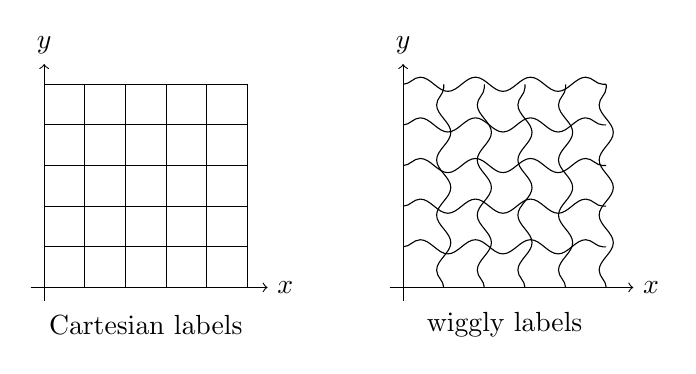
\begin{tikzpicture}[scale=0.86]
\begin{scope}
\draw[->] (-0.2,0) -- (3.3,0) node[right] {$x$};
\draw[->] (0,-0.2) -- (0,3.3) node[above] {$y$};
\foreach \u in {0.6,1.2,1.8,2.4,3.0}{
  \draw (\u,0) -- (\u,3.0);
  \draw (0,\u) -- (3.0,\u);
}
\node at (1.5,-0.55) {Cartesian labels};
\end{scope}
\begin{scope}[xshift=5.3cm]
\draw[->] (-0.2,0) -- (3.4,0) node[right] {$x$};
\draw[->] (0,-0.2) -- (0,3.3) node[above] {$y$};
\foreach \u in {0.6,1.2,1.8,2.4,3.0}{
  \draw[decorate,decoration={snake,amplitude=0.09cm,segment length=0.7cm}]
    (\u,0) -- (\u,3.0);
  \draw[decorate,decoration={snake,amplitude=0.09cm,segment length=0.7cm}]
    (0,\u) -- (3.0,\u);
}
\node at (1.5,-0.55) {wiggly labels};
\end{scope}
\end{tikzpicture}
\caption{La geometría permanece plana mientras cambia la cuadrícula de coordenadas. Las componentes de la métrica por sí solas no permiten determinar si una perturbación es física.}
\end{figure}

\section{Una onda que se propaga a lo largo del eje z}

Elijamos una onda plana que se propaga en la dirección positiva de \(z\). Su fase puede escribirse como
\begin{equation}
 k(z-t),
\end{equation}
de modo que una componente representativa tiene la forma
\begin{equation}
 h_{\mu\nu}(z,t)
 =h_{\mu\nu}^{(0)}\sin k(z-t).
 \label{eq:plane-wave}
\end{equation}
Las superficies de fase constante satisfacen \(z-t=\text{constant}\); por tanto, la velocidad de propagación es la velocidad de la luz.

En una descripción transversal y sin traza, se anulan las componentes que contienen un índice temporal o un índice \(z\):
\begin{equation}
 h_{0\mu}=0,
 \qquad
 h_{z\mu}=0.
 \label{eq:tt-transverse}
\end{equation}
Solo queda el bloque \(x\)-\(y\). Es simétrico y sin traza:
\begin{equation}
 h_{xy}=h_{yx},
 \qquad
 h_{xx}+h_{yy}=0.
 \label{eq:tt-trace}
\end{equation}

\begin{figure}[htbp]
\centering
\includegraphics[width=0.84\textwidth]{lecture_10_figure_06.png}
\caption{Una onda que se propaga a lo largo de \(z\), representada como una sucesión de planos transversales. Las amplitudes que sobreviven en \(x\)-\(y\) obedecen
\(h_{xx}+h_{yy}=0\).}
\lectureframe{00:43:36}
\end{figure}

Por tanto, hay dos patrones independientes. Para \(i,j\in\{x,y\}\), se pueden representar como
\begin{equation}
 h^{\mathrm{TT}}_{ij}(z,t)
 =
 \begin{pmatrix}
 h_+ & h_\times\\
 h_\times & -h_+
 \end{pmatrix}
 \sin k(z-t).
 \label{eq:polarization-matrix}
\end{equation}
El patrón diagonal se llama polarización plus. El patrón no diagonal se llama polarización cruzada. Una rotación de los ejes transversales de \(45^\circ\) transforma un patrón en el otro, y una onda con polarización lineal arbitraria es una superposición de ambos. En esta teoría no hay otras polarizaciones independientes.

\begin{figure}[htbp]
\centering
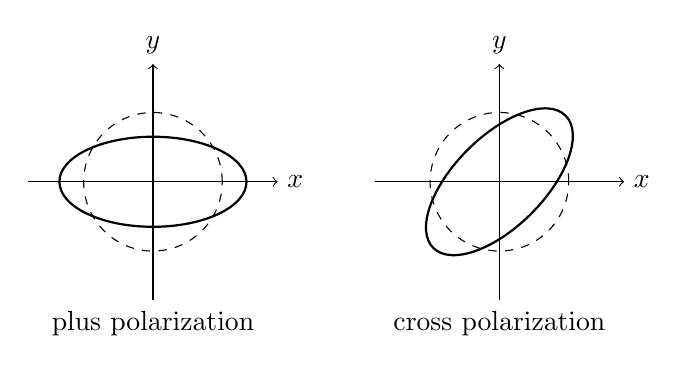
\begin{tikzpicture}[scale=0.88]
\begin{scope}
\draw[->] (-1.8,0) -- (1.8,0) node[right] {$x$};
\draw[->] (0,-1.7) -- (0,1.7) node[above] {$y$};
\draw[dashed] (0,0) circle (1.0);
\draw[thick] (0,0) ellipse (1.35 and 0.65);
\node at (0,-2.05) {plus polarization};
\end{scope}
\begin{scope}[xshift=5.0cm]
\draw[->] (-1.8,0) -- (1.8,0) node[right] {$x$};
\draw[->] (0,-1.7) -- (0,1.7) node[above] {$y$};
\draw[dashed] (0,0) circle (1.0);
\draw[thick,rotate=45] (0,0) ellipse (1.35 and 0.65);
\node at (0,-2.05) {cross polarization};
\end{scope}
\end{tikzpicture}
\caption{Durante medio ciclo, una dirección transversal se estira mientras la dirección perpendicular se contrae. Medio ciclo después, la deformación se invierte.}
\end{figure}

\section{De las componentes de la métrica a la deformación física}

Fijemos \(z\) y \(t\) y examinemos el plano transversal. Para una onda plus pura,
\begin{equation}
 ds_\perp^2
 =(1+h_{xx})\,dx^2+(1-h_{xx})\,dy^2.
 \label{eq:transverse-distance}
\end{equation}
Cuando \(h_{xx}>0\), un intervalo fijo de coordenadas en la dirección \(x\) tiene una longitud propia ligeramente mayor, mientras que el intervalo correspondiente en la dirección \(y\) tiene una longitud propia ligeramente menor. Medio período después, \(h_{xx}\) cambia de signo y se invierten los papeles. Un cuadrado se estira horizontalmente y se contrae verticalmente, y luego se contrae horizontalmente y se estira verticalmente. Para la polarización cruzada, la misma alternancia ocurre a lo largo de ejes girados \(45^\circ\).

A primer orden, un brazo que inicialmente tiene longitud \(L\) cambia en
\begin{equation}
 \frac{\Delta L}{L}\simeq\frac12 h_{ij}n^i n^j,
 \label{eq:fractional-strain}
\end{equation}
donde \(\mathbf n\) apunta a lo largo del brazo. Esta fórmula traduce la perturbación de la métrica en la deformación adimensional que mide un detector.

\begin{classroomqa}
\audiencequestion{Una regla de un metro se mantiene unida por fuerzas electromagnéticas y su longitud propia no cambia simplemente con las coordenadas. ¿No debería mostrarse en su lugar masas de prueba libres y separadas?}
\lecturerresponse{La distinción es importante. Una varilla real tiene elasticidad, por lo que el campo de marea induce tensiones en su interior; en general, una varilla de acero y una de madera responderán en distinta medida. Las masas de prueba suspendidas libremente evitan esa respuesta elástica concreta y permiten observar de forma más directa la aceleración relativa. En ambos casos, la onda que pasa no se limita a reasignar los puntos. Su curvatura dependiente del tiempo produce un efecto físico.
\lecturetimestamp{00:47:23--00:48:48}}
\end{classroomqa}

La formulación local precisa es la desviación geodésica. Para partículas cercanas en caída libre, separadas por \(\xi^i\),
\begin{equation}
 \frac{d^2\xi^i}{dt^2}
 =-R^i{}_{0j0}\,\xi^j.
 \label{eq:geodesic-deviation}
\end{equation}
En la onda débil transversal y sin traza,
\begin{equation}
 R_{0i0j}=-\frac12\ddot h^{\mathrm{TT}}_{ij},
 \label{eq:tidal-curvature}
\end{equation}
por lo que la métrica oscilante genera una aceleración de marea alternante. Por eso no se puede descartar una onda dependiente del tiempo como una elección estática de reglas de medir. Tiene curvatura no nula.

\begin{classroomqa}
\audiencequestion{¿Qué puede medir la contracción y el estiramiento si todas las reglas de la región se ven afectadas?}
\lecturerresponse{Un extensómetro puede registrar la tensión real inducida en un cuerpo material. Mejor aún, se puede monitorizar la separación cambiante entre masas suspendidas libremente. Una reescala estática y uniforme podría incorporarse al aparato de medida, pero la curvatura oscilante provoca una respuesta que puede registrarse.
\lecturetimestamp{00:51:10--00:52:02}}
\end{classroomqa}

\section{Fuentes y detectores}

Las ondas electromagnéticas las generan cargas y corrientes en movimiento. Las ondas gravitacionales las generan distribuciones de masa y energía en movimiento. La conservación de la energía y del momento descarta la radiación gravitacional monopolar y dipolar en un sistema aislado, por lo que el primer momento radiativo es cuadrupolar. Un sistema binario compacto proporciona precisamente el cuadrupolo variable necesario: dos cuerpos densos orbitan uno alrededor del otro y emiten ondas hacia el campo lejano.

Cerca del sistema binario, el espacio-tiempo está fuertemente curvado y la expansión lineal de la ecuación~\eqref{eq:weak-split} no es fiable. Lejos de allí, la onda saliente se propaga sobre un área mayor, su amplitud disminuye y la descripción linealizada se vuelve precisa. Para un observador situado sobre el eje \(z\) respecto de la fuente, el estiramiento medible se produce en el plano transversal \(x\)-\(y\).

\begin{classroomqa}
\audiencequestion{¿La regla del dibujo representa una regla abstracta de coordenadas o una regla física de un metro? ¿Y cómo podría una regla variable medir el efecto?}
\lecturerresponse{Puede ser un objeto físico, pero entonces importan sus propiedades materiales. La curvatura produce la tensión de marea; el acero y la madera no tienen por qué deformarse del mismo modo. Comparar sus respuestas ya constituye una medición. Un detector más limpio sustituye las varillas por masas de prueba separadas y mide su movimiento diferencial.
\lecturetimestamp{00:54:00--00:55:19}}
\end{classroomqa}

Un detector resonante es una estrategia. Si un sistema mecánico tiene una frecuencia natural cercana a la de la onda incidente, esta lo impulsa coherentemente y amplifica la respuesta. Un interferómetro emplea otra estrategia: los espejos actúan como masas de prueba y la interferencia láser compara las longitudes efectivas de brazos perpendiculares. Una onda polarizada en modo plus alarga un brazo mientras acorta el otro, lo que produce precisamente la señal diferencial que un interferómetro está diseñado para detectar.

\begin{classroomqa}
\audiencequestion{¿Esta podría ser la base de un detector de ondas gravitacionales?}
\lecturerresponse{Sí. Una varilla rígida apenas cambia, mientras que las masas de prueba de los extremos, suspendidas libremente, pueden experimentar aceleración relativa. También se puede aprovechar la resonancia para que un impulso periódico débil produzca una respuesta mayor. La deformación astrofísica prevista es extraordinariamente pequeña, del orden de \(10^{-21}\), así que diseñar detectores consiste en convertir ese movimiento diferencial diminuto en una señal medible.
\lecturetimestamp{00:55:20--00:57:10}}
\end{classroomqa}

\begin{classroomqa}
\audiencequestion{¿LIGO es un ejemplo de ese tipo de detector?}
\lecturerresponse{Sí. Sus observables básicos se obtienen con luz láser reflejada entre espejos situados en brazos perpendiculares. Una onda gravitacional cambia las longitudes relativas de los recorridos ópticos y, por tanto, el patrón de interferencia. En el momento de esta clase, el instrumento todavía no había realizado una detección directa; esa situación histórica cambió más adelante.\editorialnote{La primera observación directa, GW150914, se registró en 2015 y se anunció en 2016.}
\lecturetimestamp{00:57:16--00:58:05}}
\end{classroomqa}

\begin{classroomqa}
\audiencequestion{¿Qué velocidad de propagación se deduce de la solución ondulatoria?}
\lecturerresponse{La velocidad de la luz. La fase \(k(z-t)\) se desplaza una unidad en \(z\) por cada unidad en \(t\), y la ecuación de Einstein linealizada tiene la misma estructura de propagación sobre el cono de luz que la ecuación de ondas electromagnéticas.
\lecturetimestamp{00:58:07--00:58:16}}
\end{classroomqa}

Las colisiones de agujeros negros y los sistemas binarios compactos son fuentes especialmente prometedoras. Cerca de la colisión, el campo gravitacional es intensamente no lineal, y una parte considerable de la energía liberada puede salir como radiación gravitacional. Cuando la señal llega a un detector distante, su amplitud ya es lo bastante débil como para que la propagación lineal de ondas constituya una descripción excelente. Así, la radiación gravitacional abre un canal astronómico que no tiene por qué depender de la luz emitida.

\section{El púlsar binario y las pruebas indirectas}

La radiación transporta energía. Si un sistema binario emite ondas gravitacionales, su energía orbital disminuye, los cuerpos se acercan lentamente en espiral y el período orbital cambia. El púlsar binario proporciona un reloj lo bastante preciso para medir ese cambio. La evolución orbital observada concuerda cuantitativamente con la pérdida de energía predicha por la relatividad general.

En el contexto histórico de la clase, esta era la prueba indirecta decisiva: ningún detector había registrado aún una onda al pasar por la Tierra, pero la órbita perdía energía a la tasa que exige la radiación gravitacional. Las ondas ya se podían observar por el efecto que tenían en su fuente.

\begin{classroomqa}
\audiencequestion{¿Qué frecuencia o período caracteriza al sistema original del púlsar binario? ¿Es del orden de los milisegundos?}
\lecturerresponse{La escala de milisegundos se refiere al giro del púlsar, no a la órbita de las dos estrellas. En clase se comprueba el valor y se obtiene un período orbital de aproximadamente \(7.75\) horas. La distinción importa: la radiación gravitacional sigue el movimiento orbital del sistema binario, mientras que los pulsos de radio proporcionan el reloj preciso con que se lo estudia.
\lecturetimestamp{01:01:27--01:03:28}}
\end{classroomqa}

\begin{classroomqa}
\audiencequestion{¿Cuánto cambió el tiempo orbital acumulado durante las décadas de observación?}
\lecturerresponse{El desplazamiento acumulado citado es de unos treinta segundos. El cambio fraccional instantáneo es diminuto, pero décadas de cronometraje preciso de los pulsos hacen visible el efecto acumulado.
\lecturetimestamp{01:03:34--01:03:54}}
\end{classroomqa}

\section{Dependencia temporal, curvatura y límites de la linealidad}

\begin{classroomqa}
\audiencequestion{¿Por qué elegir el plano transversal \(x\)-\(y\)? ¿Qué ocurre si, en cambio, se considera un plano que incluya \(x\) y \(t\)?}
\lecturerresponse{La onda misma depende de \(z\) y \(t\), pero «transversal» se refiere a las direcciones espaciales perpendiculares a su dirección espacial de propagación. Para una onda que se propaga a lo largo de \(z\), las amplitudes métricas físicas pueden elegirse en el bloque \(x\)-\(y\). Las demás componentes aparentes son oscilaciones de coordenadas que no están presentes o que pueden eliminarse.
\lecturetimestamp{01:02:22--01:03:17}}
\end{classroomqa}

\begin{classroomqa}
\audiencequestion{¿Oscila el tiempo mismo?}
\lecturerresponse{No. La onda oscila en función del tiempo. En una posición espacial fija, las componentes \(h_{ij}(z,t)\) varían periódicamente. En esta descripción, el tiempo es una coordenada de la que depende el campo, no un objeto que se estire y se comprima alternativamente.
\lecturetimestamp{01:04:00--01:04:18}}
\end{classroomqa}

\begin{classroomqa}
\audiencequestion{Si todas las componentes \(h_{0\mu}\) se anulan, ¿no hay curvatura que involucre la dirección temporal?}
\lecturerresponse{Sí la hay. Las componentes espaciales que sobreviven dependen del tiempo, y la curvatura contiene dos derivadas de ellas. Por tanto, derivadas como \(\partial_t^2h_{ij}\) generan componentes \(R_{0i0j}\). Que se anulen las componentes de \(h_{\mu\nu}\) con índices temporales no implica que la curvatura dependiente del tiempo también se anule.
\lecturetimestamp{01:05:15--01:06:09}}
\end{classroomqa}

La ecuación de ondas lineal surgió porque se supuso que \(h\) era pequeño, no porque se eliminaran los artefactos de coordenadas. Son dos operaciones distintas. La fijación del gauge identifica los grados de libertad físicos; la linealización descarta las interacciones no lineales.

\begin{classroomqa}
\audiencequestion{Las ecuaciones de Einstein son no lineales, pero la ecuación de ondas resultante es lineal. ¿Se debe esa linealidad a la eliminación de las soluciones no físicas?}
\lecturerresponse{No. Se debe a la aproximación de amplitud pequeña. Se descartaron los términos que contienen dos potencias de \(h\). Eliminar las oscilaciones de coordenadas determina qué soluciones son físicas; no es lo que vuelve lineal la ecuación.
\lecturetimestamp{01:06:45--01:07:29}}
\end{classroomqa}

\begin{classroomqa}
\audiencequestion{Una vez resuelta la ecuación linealizada, ¿qué magnitud tiene el error respecto de una solución exacta?}
\lecturerresponse{Las primeras correcciones omitidas son del orden de \(h^2\). Si \(h\sim10^{-1}\), son del orden de \(10^{-2}\); si \(h\sim10^{-3}\), son del orden de \(10^{-6}\). Después, siempre hay que comprobar el cálculo perturbativo para asegurarse de que el parámetro que se supuso pequeño realmente lo era.
\lecturetimestamp{01:07:35--01:08:31}}
\end{classroomqa}

\begin{classroomqa}
\audiencequestion{Cuando los términos de orden superior se vuelven importantes, ¿pierde la onda su carácter transversal?}
\lecturerresponse{Se conserva el carácter transversal esencial de la radiación, pero no la superposición lineal. Las ondas intensas interactúan con el campo gravitacional transportado por otras ondas; en lugar de atravesarse sin cambios, se dispersan.
\lecturetimestamp{01:08:34--01:09:11}}
\end{classroomqa}

\begin{classroomqa}
\audiencequestion{La velocidad de una onda mecánica depende de la rigidez y de la densidad. ¿Hay un sentido comparable en que el espacio-tiempo tenga rigidez?}
\lecturerresponse{Solo por analogía. En un medio material, la propagación depende de una combinación como la rigidez dividida por la densidad. Como las ondas electromagnéticas y gravitacionales se propagan a \(c\), el lenguaje mecánico antiguo describiría su medio como extraordinariamente rígido. La física moderna no atribuye al espacio-tiempo un módulo de Young ordinario; el hecho invariante es la propagación a la velocidad de la luz que fijan las ecuaciones de campo.
\lecturetimestamp{01:09:12--01:11:10}}
\end{classroomqa}

\section{Una segunda vía: acción estacionaria}

Terminada la discusión de las ondas, queda tiempo para un último cambio de perspectiva. El principio de acción estacionaria es el lenguaje común de la mecánica clásica, el electromagnetismo, la teoría de campos y el modelo estándar. La relatividad general forma parte de la misma estructura.

Para una partícula, la acción es una integral a lo largo de una trayectoria. Para un campo, una historia asigna un valor del campo \(\phi(x)\) a cada punto del espacio-tiempo, y la acción es una integral sobre el espacio-tiempo:
\begin{equation}
 S[\phi]
 =\int d^4x\,
 \mathcal L\bigl(\phi,\partial_\mu\phi\bigr).
 \label{eq:field-action}
\end{equation}
Cualquier \(\phi(x)\) suficientemente regular es una historia concebible, del mismo modo que cualquier trayectoria suficientemente regular es una trayectoria concebible para una partícula, pero la mayoría no son soluciones. Las historias físicas son puntos estacionarios de la acción, con datos de contorno fijos:
\begin{equation}
 \delta S=0.
 \label{eq:stationary-action}
\end{equation}
Para un campo, el contorno rodea una región del espacio-tiempo, en vez de limitarse a especificar los dos extremos de una trayectoria. Las ecuaciones de Euler--Lagrange seleccionan entonces la interpolación entre los valores de contorno prescritos.

Las ecuaciones de campo de Einstein se pueden obtener exactamente de este modo. La variación es larga, pero la acción misma es sencilla. Antes de escribirla, necesitamos la medida apropiada de volumen del espacio-tiempo.

\section{Por qué el determinante mide el volumen}

Empecemos en dos dimensiones con una métrica diagonal:
\begin{equation}
 ds^2=g_{xx}\,dx^2+g_{yy}\,dy^2.
\end{equation}
Un rectángulo de coordenadas con lados \(dx\) y \(dy\) tiene longitudes propias de lado \(\sqrt{g_{xx}}\,dx\) y \(\sqrt{g_{yy}}\,dy\), así que su área propia es
\begin{equation}
 dA
 =\sqrt{g_{xx}g_{yy}}\,dx\,dy.
\end{equation}
Si está presente la componente no diagonal \(g_{xy}\), los lados coordenados no tienen por qué ser ortogonales. El área corregida es
\begin{equation}
 dA
 =\sqrt{g_{xx}g_{yy}-g_{xy}^2}\,dx\,dy
 =\sqrt{\det g}\,dx\,dy.
 \label{eq:area-determinant}
\end{equation}

\begin{figure}[htbp]
\centering
\includegraphics[width=0.84\textwidth]{lecture_10_figure_07.png}
\caption{La generalización en la pizarra, desde un pequeño rectángulo de coordenadas hasta el elemento de área propia \(\sqrt{\lvert g\rvert}\,dx\,dy\). El determinante incorpora tanto las longitudes diagonales como el cizallamiento no diagonal.}
\lectureframe{01:21:25}
\end{figure}

La misma construcción funciona en cualquier dimensión:
\begin{equation}
 dV_n=\sqrt{|\det g|}\,d^nx.
\end{equation}
Para el espacio-tiempo lorentziano, si \(g=\det(g_{\mu\nu})\), el elemento invariante de volumen cuatridimensional se escribe convencionalmente como
\begin{equation}
 dV_4=\sqrt{|g|}\,d^4x,
 \label{eq:four-volume}
\end{equation}
o como \(\sqrt{-g}\,d^4x\) en la convención de signatura mayormente positiva. Las coordenadas de una región pueden cambiar, pero su volumen físico cuatridimensional no.

Multiplicar esta medida por cualquier escalar \(F(x)\) e integrar produce una cantidad invariante bajo cambios de coordenadas:
\begin{equation}
 \int d^4x\,\sqrt{|g|}\,F(x).
 \label{eq:invariant-scalar-integral}
\end{equation}
Una acción para una teoría generalmente covariante debería tener esta forma. De lo contrario, las ecuaciones de campo que se obtuvieran de ella podrían depender de una elección arbitraria de coordenadas.

\section{Acción de Einstein--Hilbert}

En la gravedad pura, el campo dinámico es la propia métrica. El escalar no constante más sencillo que se construye a partir de la métrica y sus dos primeras derivadas es el escalar de curvatura \(R\). Una constante también es un escalar; su coeficiente es la constante cosmológica. Salvo por convenciones de signo y términos de contorno, una normalización estándar de la acción gravitacional es
\begin{equation}
 S_{\mathrm{grav}}
 =
 \frac{1}{16\pi G}
 \int d^4x\,\sqrt{|g|}\,(R-2\Lambda).
 \label{eq:einstein-hilbert}
\end{equation}

\begin{figure}[htbp]
\centering
\includegraphics[width=0.84\textwidth]{lecture_10_figure_08.png}
\caption{La representación de la historia del campo y la acción gravitacional en la pizarra. El escalar de curvatura proporciona la dinámica; el término constante es proporcional al volumen del espacio-tiempo.}
\lectureframe{01:26:32}
\end{figure}

El término proporcional a \(\Lambda\) es simplemente un múltiplo del volumen total del espacio-tiempo. La ecuación de ondas anterior se desarrolló para el vacío con \(\Lambda=0\), así que ese término no aparecía allí.

La materia se incorpora mediante una acción de materia:
\begin{equation}
 S=S_{\mathrm{grav}}+S_{\mathrm{matter}}.
\end{equation}
Por ejemplo, en el electromagnetismo, la contribución invariante del campo se construye a partir del tensor antisimétrico \(F_{\mu\nu}\):
\begin{equation}
 S_{\mathrm{EM}}
 =-\frac14
 \int d^4x\,\sqrt{|g|}\,
 F_{\mu\nu}F^{\mu\nu}.
\end{equation}
La variación de la acción total con respecto a la métrica inversa define el tensor de energía-momento y da
\begin{equation}
 R_{\mu\nu}
 -\frac12 g_{\mu\nu}R
 +\Lambda g_{\mu\nu}
 =8\pi G\,T_{\mu\nu}.
 \label{eq:einstein-from-action}
\end{equation}
Así, la acción compacta contiene las ecuaciones de campo completas. En el vacío, con \(\Lambda=0\), se reduce a la teoría que gobernaba las ondas gravitacionales estudiadas antes.

\begin{classroomqa}
\audiencequestion{¿Dónde entra el tensor de energía-momento en el principio de acción?}
\lecturerresponse{Proviene de los términos adicionales que describen la materia y otros campos. La energía electromagnética, los campos de partículas y cualquier otro contenido material contribuyen a \(S_{\mathrm{matter}}\). Su variación respecto de la métrica proporciona \(T_{\mu\nu}\). La integral que contiene únicamente \(\sqrt{|g|}R\) constituye la teoría gravitatoria en el vacío.
\lecturetimestamp{01:27:26--01:28:25}}
\end{classroomqa}

La derivación es conceptualmente sencilla, pero algebraicamente desagradable. Se construyen los símbolos de Christoffel a partir de la métrica, se construye la curvatura, se contrae para formar \(R\), se multiplica por el factor del determinante y se varía la expresión resultante. En la clase se bromea con que el ejercicio debería llevar cinco minutos y que, si no se logra, se suspendería el curso; acto seguido, se admite que se ha abandonado el cálculo muchas veces tras intentarlo durante mucho más tiempo. La broma apunta a algo serio: que los principios sean compactos no implica que los cálculos por componentes sean breves.

\begin{classroomqa}
\audiencequestion{¿Se suele escribir completa la variación en un texto de relatividad?}
\lecturerresponse{Se puede hacer, pero ocupa páginas. Un cálculo largo solo resulta esclarecedor cuando se trabaja lo suficiente como para entender por qué se sigue el paso siguiente; leer pasivamente línea tras línea rara vez permite alcanzar esa comprensión. Las herramientas simbólicas y numéricas modernas pueden encargarse de buena parte de las operaciones algebraicas, pero no sustituyen el principio organizador.
\lecturetimestamp{01:31:10--01:34:16}}
\end{classroomqa}

Hay dos maneras tradicionales de abordar estos cálculos. Se puede desarrollar una intuición geométrica lo bastante sólida como para reconocer qué combinaciones de tensores son posibles, o se puede avanzar con cuidado por el álgebra. La mayoría de los trabajos combina ambos enfoques en alguna medida y, a menudo, se deja que un ordenador realice las contracciones más largas. En el curso se han destacado deliberadamente los principios que se mantienen, cualquiera que sea el método elegido.

\begin{classroomqa}
\audiencequestion{A posteriori, la acción parece estar muy bien motivada. ¿Por qué le llevó tantos años a Einstein pasar de la relatividad especial a la relatividad general, y desde el principio aspiraba a llegar a la teoría final?}
\lecturerresponse{El punto de llegada parece más sencillo una vez conocida la geometría necesaria. En aquella época, la mayoría de los físicos no estaba familiarizada con la geometría diferencial necesaria, y Einstein tuvo que aprenderla y adaptarla con ayuda matemática, en particular de Marcel Grossmann. Construir los conceptos de espacio-tiempo curvo y hallar la ecuación de campo correcta en aproximadamente una década no fue un logro lento. Vale la pena leer los artículos iniciales y los finales precisamente porque muestran cuánto hubo que inventar en el camino.
\lecturetimestamp{01:34:20--01:35:59}}
\end{classroomqa}

El trimestre termina, por tanto, con dos formulaciones complementarias de una misma teoría. La ecuación de campo indica cómo responde localmente la curvatura al tensor de energía-momento. El principio de acción afirma que toda la historia del espacio-tiempo es un punto estacionario de un único funcional invariante. En el campo lejano débil, ambas descripciones se reducen a ondas transversales que transportan curvatura real a la velocidad de la luz.